\documentclass[12pt]{article}
\usepackage[table]{xcolor}
\usepackage[shortlabels]{enumitem}
\usepackage{tabularx,xltabular}
\usepackage{graphicx}
\usepackage{hyperref}
\usepackage{verbatim}
\usepackage{geometry}
\usepackage{ulem}
\usepackage[official]{eurosym}
\usepackage{tikz}
\usetikzlibrary{arrows,backgrounds,calc,decorations.markings,patterns,3d,positioning,fit,angles, quotes}
\usepackage{pgfplots}
\pgfplotsset{compat = newest}
\usetikzlibrary{fit}
\newcommand\addvmargin[1]{
\usetikzlibrary{arrows}
\node[fit=(current bounding box),inner ysep=#1,inner xsep=0]{};}
\usepackage{cancel}
\usepackage{fontspec}
\usepackage{array}  
\geometry{a4paper, top=2cm, left=2cm, right=2cm, bottom=2cm, headsep=1cm}
\usepackage{tabu}
\usepackage{pst-node}
\usepackage{colortbl}
\usepackage{array}
\usepackage{german}
\setlength\parindent{0pt}
\newcolumntype{?}{!{\vrule width 1pt}}
\usepackage{makecell}
\renewcommand{\arraystretch}{2.5}
\usepackage{pbox}
\usepackage{amssymb}
\usepackage{amsmath}
\usepackage{booktabs}
\newcolumntype{L}[1]{>{\raggedright\let\newline\\\arraybackslash\hspace{0pt}}m{#1}}
\newcolumntype{C}[1]{>{\centering\let\newline\\\arraybackslash\hspace{0pt}}m{#1}}
\newcolumntype{R}[1]{>{\raggedleft\let\newline\\\arraybackslash\hspace{0pt}}m{#1}}
\begin{document}
\rightline{Datum: 12.12.2023}
\centerline{{\Large Flächen und Umfänge}} 
\vspace{1cm}
\noindent \\


\begin{xltabular}{\textwidth}{|C{0.75cm}|X|C{0.75cm}|X|}
\arrayrulecolor{black}\hline
a)&Setze für die Variabel a den Wert -4 ein und berechne den Wert des Terms:$$2 + a$$
&
b)&Setze für die Variabel a den Wert -6 ein und berechne den Wert des Terms:$$4 \cdot a - 4 \cdot a$$
\\\hline
c)&Vereinfache:$$4b - 5b - 2=?$$
&
d)&Vereinfache:$$b + 2 - b=?$$
\\\hline
e)&Berechne die Variable $$x-42 = 40$$
&
f)&Berechne die Variable $$4\cdot a=24$$
\\\hline
g)&Berechne die Variable $$3\cdot b-4=32$$
&
h)&\pbox{6cm}{Bestimme den Umfang und die Fläche von: \\\tikzstyle{background grid}=[draw, black!15,step=.5cm]
\noindent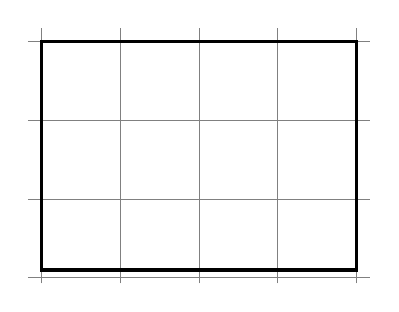
\begin{tikzpicture}[show background grid]
\draw[black, very thick] (0cm,0.1cm) rectangle (4cm,3cm);
\end{tikzpicture}}
\\\hline
i)&\pbox{5cm}{
Berechne den Flächeninhalt von:\\
\tikzstyle{background grid}=[draw, black!15,step=.5cm]
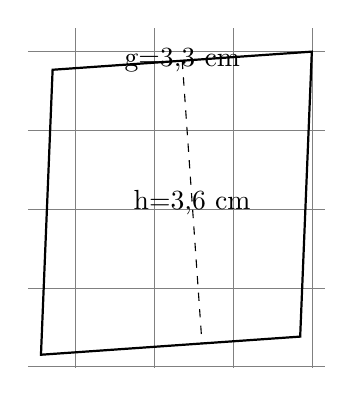
\begin{tikzpicture}[show background grid]
\draw[thick,black,rotate=184] (0,0) -- node{g=3,3 cm} ++(3.3,0) -- ++(0.4,3.6) -- ++(-3.3,0) --cycle;
\draw[dashed,black,rotate=184] (1.65,0)  -- node{h=3,6 cm} ++(0,3.6);
\end{tikzpicture}
}
&
j)&\pbox{5cm}{
Berechne den Flächeninhalt von:\\
\tikzstyle{background grid}=[draw, black!15,step=.5cm]
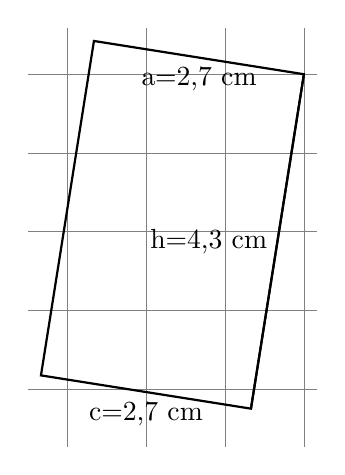
\begin{tikzpicture}[show background grid]
\draw[thick,black,rotate=171] (0,0) -- node[below]{a=2,7 cm} ++(2.7,0) -- ++(-0.0,4.3) --node[below]{c=2,7 cm} ++(-2.7,0) --cycle;
\draw[thick,black,rotate=171] (0.0,0) --node[left]{h=4,3 cm}  ++(0,4.3);
\end{tikzpicture}
}
\\\hline
k)&\pbox{5cm}{
Berechne den Flächeninhalt von:\\
\tikzstyle{background grid}=[draw, black!15,step=.5cm]
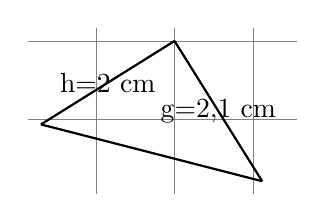
\begin{tikzpicture}[show background grid]
\draw[thick,black] (122:-2.1) -- node{g=2,1 cm} (122:0.0);
\draw[thick,black] (122:-2.1)  -- (212:2.0);
\draw[thick,black] (122:0.0)  -- (212:2.0);
\draw[dashed,black] (0,0)  -- node{h=2 cm} (212:2.0);
\draw[dashed,black] (0,0)  -- (122:-2.1);
\end{tikzpicture}
}
&
l)&Stelle die Flächenformel des Rechtecks nach der fehlenden Seite um und berechne diese und den Umfang für $A=82,65~cm^2$ und $a=8,7~cm$.
\\\hline
m)&Stelle die Umfangsformel des Parallelogramm nach der fehlenden Seite um und berechne diese und den Flächeninhalt für $u=35,8~cm$, $b=8~cm$ und $h_a=8,5 cm$.
&
\end{xltabular}
\vspace{0.5cm}
\newpage
\rightline{Datum: 12.12.2023}
\centerline{{\large Lösungen Flächen und Umfänge}} 
\vspace{0.5cm}

\begin{xltabular}{\textwidth}{|C{0.75cm}|X|C{0.75cm}|X|}
\arrayrulecolor{black}\hline
a)&$\begin{aligned}
\textcolor{red}{a=-4} & \rightarrow\\
2 + a=&2 + \textcolor{red}{(-4)}=-2\\
\end{aligned}$
&
b)&$\begin{aligned}
\textcolor{red}{a=-6} & \rightarrow\\
4 \cdot a - 4 \cdot a=&4 \cdot \textcolor{red}{(-6)} - 4 \cdot \textcolor{red}{(-6)}=0\\
\end{aligned}$
\\\hline
c)&$4b - 5b - 2=-b - 2$
&
d)&$b + 2 - b=2$
\\\hline
e)&\begingroup\setlength{\jot}{-0.03cm}
\tikzstyle{background grid}=[draw, black!15,step=.5cm]
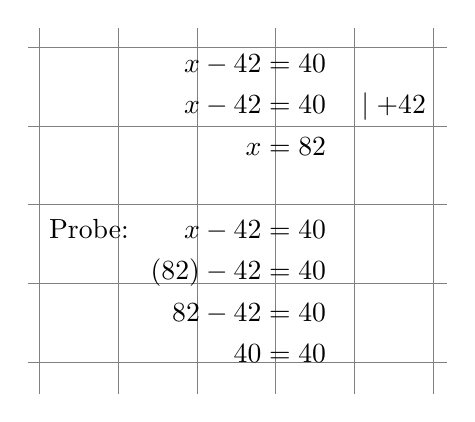
\begin{tikzpicture}[show background grid]
\node[below right] at (0,0.1) {
$\begin{aligned}
x-42  &= 40& &  \\
x - 42 &=40& & \mid + 42\\
x &=82& & 
\\
\\
\mbox{Probe:}\qquad x-42  &= 40& &  \\
\left(82\right)-42  &= 40& &  \\
82-42 &=40& &  \\
40 &=40& &  \\
\end{aligned}$};
\end{tikzpicture}
\endgroup
&
f)&\begingroup\setlength{\jot}{-0.03cm}
\tikzstyle{background grid}=[draw, black!15,step=.5cm]
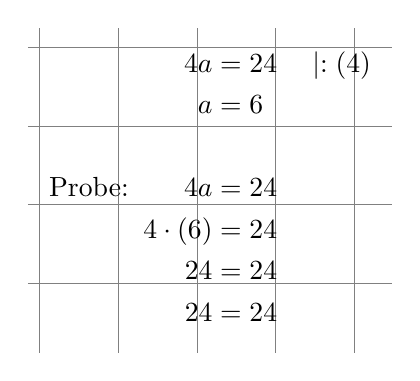
\begin{tikzpicture}[show background grid]
\node[below right] at (0,0.1) {
$\begin{aligned}
4a &=24& & \mid :\left(4\right)\\
a &=6& & 
\\
\\
\mbox{Probe:}\qquad 4a &=24& &  \\
4\cdot \left(6\right) &=24& &  \\
24 &=24& &  \\
24 &=24& &  \\
\end{aligned}$};
\end{tikzpicture}
\endgroup
\\\hline
g)&\begingroup\setlength{\jot}{-0.03cm}
\tikzstyle{background grid}=[draw, black!15,step=.5cm]
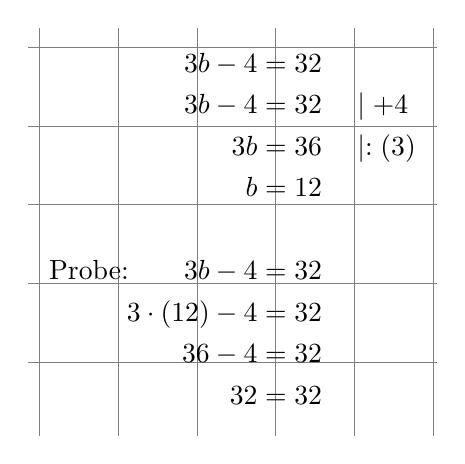
\begin{tikzpicture}[show background grid]
\node[below right] at (0,0.1) {
$\begin{aligned}
3b-4 &=32& &  \\
3b - 4 &=32& & \mid + 4\\
3b &=36& & \mid :\left(3\right)\\
b &=12& & 
\\
\\
\mbox{Probe:}\qquad 3b-4 &=32& &  \\
3\cdot \left(12\right)-4 &=32& &  \\
36-4 &=32& &  \\
32 &=32& &  \\
\end{aligned}$};
\end{tikzpicture}
\endgroup
&
h)&\pbox{6cm}{$U=2\cdot a+2\cdot b$ \\ $U=2\cdot4cm+2\cdot3cm=14cm$ \\$A=a\cdot b$ \\ $A=4\cdot3=12cm^2$ \\\tikzstyle{background grid}=[draw, black!15,step=.5cm]
\noindent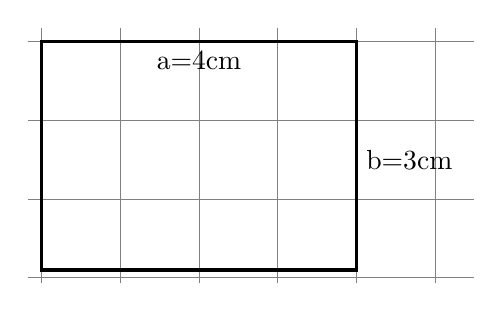
\begin{tikzpicture}[show background grid]
\draw[black, very thick] (0cm,0.1cm) rectangle (4cm,3cm);
\draw (2.0cm,3cm) node[below]{a=4cm}; 
\draw (4cm,1.5cm) node[right]{b=3cm}; 
\end{tikzpicture}}
\\\hline
i)&\pbox{5cm}{
$\begin{aligned}
geg.: g&=3,3 cm \\
   h&=3,6 cm \\
ges.: A&=? \\
A&=g\cdot h \\
&=3,3\cdot 3,6 \\
\makebox[0pt][l]{\uuline{\phantom{$A=11,88~cm^2$} } }
A&=11,88~cm^2
\end{aligned}$
\tikzstyle{background grid}=[draw, black!15,step=.5cm]
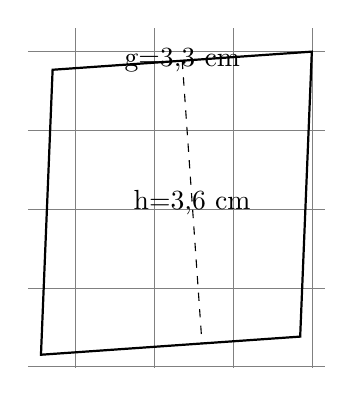
\begin{tikzpicture}[show background grid]
\draw[thick,black,rotate=184] (0,0) -- node{g=3,3 cm} ++(3.3,0) -- ++(0.4,3.6) -- ++(-3.3,0) --cycle;
\draw[dashed,black,rotate=184] (1.65,0)  -- node{h=3,6 cm} ++(0,3.6);
\end{tikzpicture}
}
&
j)&\pbox{5cm}{
\tikzstyle{background grid}=[draw, black!15,step=.5cm]
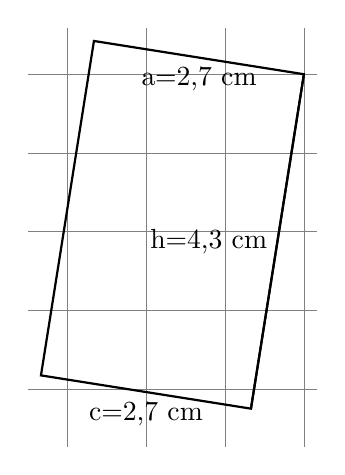
\begin{tikzpicture}[show background grid]
\draw[thick,black,rotate=171] (0,0) -- node[below]{a=2,7 cm} ++(2.7,0) -- ++(-0.0,4.3) --node[below]{c=2,7 cm} ++(-2.7,0) --cycle;
\draw[thick,black,rotate=171] (0.0,0) --node[left]{h=4,3 cm}  ++(0,4.3);
\end{tikzpicture}
$\begin{aligned}
geg.: a&=2,7 cm \\
   c&=2,7 cm \\
   h&=4,3 cm \\
ges.: A&=? \\
A&=\frac{a+c}{2}\cdot h \\
&=\frac{2,7+2,7}{2}\cdot4,3\\
\makebox[0pt][l]{\uuline{\phantom{$A=11,61~cm^2$} } }
A&=11,61~cm^2
\end{aligned}$
}
\\\hline
k)&\pbox{5cm}{
$\begin{aligned}
geg.: g&=2,1 cm \\
   h&=2 cm \\
ges.: A&=? \\
A&=\frac{g \cdot h}{2} \\
&=2,1 \cdot \frac{2}{2}\\
\makebox[0pt][l]{\uuline{\phantom{$A=2,1~cm^2$} } }
A&=2,1~cm^2
\end{aligned}$
\tikzstyle{background grid}=[draw, black!15,step=.5cm]
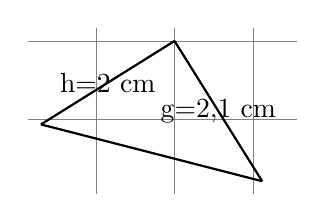
\begin{tikzpicture}[show background grid]
\draw[thick,black] (122:-2.1) -- node{g=2,1 cm} (122:0.0);
\draw[thick,black] (122:-2.1)  -- (212:2.0);
\draw[thick,black] (122:0.0)  -- (212:2.0);
\draw[dashed,black] (0,0)  -- node{h=2 cm} (212:2.0);
\draw[dashed,black] (0,0)  -- (122:-2.1);
\end{tikzpicture}
}
&
l)&\tikzstyle{background grid}=[draw, black!15,step=.5cm]
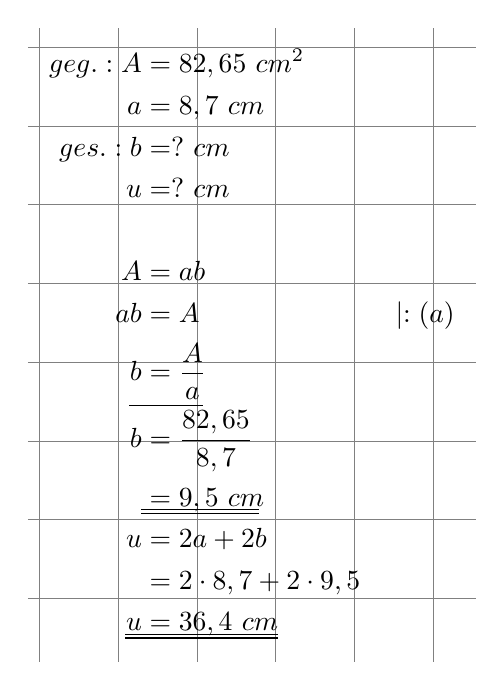
\begin{tikzpicture}[show background grid]
\node[below right] at (0,0.1) {
$\begin{aligned}
geg.: A &=82,65~cm^2& & \\
  a &=8,7~cm& & \\
ges.: b &=?~cm& & \\
u &=?~cm& & \\
& & & \\
A &=ab& & \\
ab &=A& & \mid :(a)\\
\makebox(0pt,-0.25cm)[l]{\uline{\phantom{$b ={{\frac{A}{a}}}  \\$}}}
b &={{\frac{A}{a}}}& & \\
b&=\frac{82,65}{8,7}& & \\
\makebox[0pt][l]{\uuline{\phantom{$=9,5~cm  \\$}}}
&=9,5~cm& & \\
u&=2a+2b & & \\
&=2\cdot8,7+2\cdot9,5& & \\
\makebox[0pt][l]{\uuline{\phantom{$u=36,4~cm     \\$}}}
u&=36,4~cm   & & \\
\end{aligned}$};
\end{tikzpicture}
\\\hline
m)&\tikzstyle{background grid}=[draw, black!15,step=.5cm]
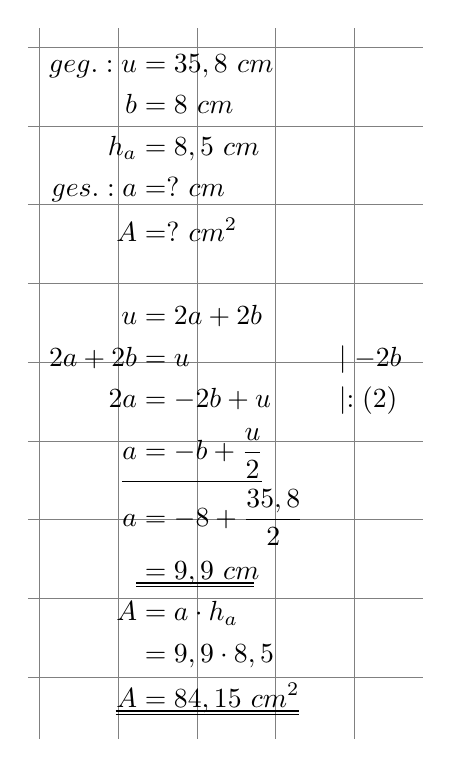
\begin{tikzpicture}[show background grid]
\node[below right] at (0,0.1) {
$\begin{aligned}
geg.: u &=35,8~cm& & \\
  b &=8~cm& & \\
 h_a &=8,5~cm& & \\
ges.: a &=?~cm& & \\
A &=?~cm^2& & \\
& & & \\
u &=2a+2b& & \\
2a + 2b &=u& & \mid - 2b\\
2a &=-2b + u& & \mid :(2)\\
\makebox(0pt,-0.25cm)[l]{\uline{\phantom{$a =-b +{{\frac{ u}{2}}}  \\$}}}
a &=-b +{{\frac{ u}{2}}}& & \\
a&=-8+\frac{35,8}{2}& & \\
\makebox[0pt][l]{\uuline{\phantom{$=9,9~cm  \\$}}}
&=9,9~cm& & \\
A&=a\cdot h_a & & \\
&=9,9\cdot8,5& & \\
\makebox[0pt][l]{\uuline{\phantom{$A=84,15~cm^2     \\$}}}
A&=84,15~cm^2   & & \\
\end{aligned}$};
\end{tikzpicture}
&
\end{xltabular}
\vspace{0.5cm}
\end{document}